\chapter{Performance} 
	Unless otherwise specified the following tests were performed using two CPUs or two GPUs, with MPI as the interface between multiple threads. The machine specifications are as follows:
\begin{itemize}
	\item CPU: Intel Core i7 930 @ 2.8GHz.
	\item Memory: 12GB (3 x 4GB) DDR3 - 1333MHz ECC Unbuffered Server memory. 
	\item GPUs: 2x EVGA GeForce GTX 470 1280MB, 607 MHz / 1215 MHz, Graphics / Processor Clock. 
	\item Motherboard: ASUS P6T7 WS Cupercomputer Intel x58.
\end{itemize}
%	\section{Test Setup}
%		\subsection{Parameter Space Explored}
%		\subsection{Machine Parameters}
%		\subsection{Memory Bandwidth Comparison}

Typical total\footnote[1]{Total run time includes MPI reduces and various other subroutines that were not ported to the GPU} speedups on this setup are on the order of 40x. A detailed breakdown of the run times per particle per time step and the speedup achieved by the GPU can be seen in table \ref{tab:speedup}. This run was performed on 2 GPUs with 17 million particles per GPU and a grid size of $64^3$.
\noindent \begin{table}[h]
\begin{tabular}{| p{4.0cm} | p{3.5cm} | p{2.5cm} | p{4.0cm} |}
\hline
Component & CPU (ns) & GPU (ns) & Speedup \\ \hline
Sort & 0 & 1.428 & - \\ \hline
Charge Assign & 150.265 & 0.577 & 260x \\ \hline
Charge Assign \& Sort & 150.265 & 2.005 & 75x \\ \hline
Poisson Solve & 40.347 & 3.045 & 13x \\ \hline
Particle Advance & 188.177 & 2.475 & 76x \\ \hline
Total\footnote[1] & 380.635 & 8.695 & 44x \\ \hline
\end{tabular}
\caption{CPU and GPU Runtime comparison for 2 GTX 470's vs an Intel(R) Core i7 930 Test was performed using 2 MPI threads handling 17 million particles each on a $64^3$ grid.}
\label{tab:speedup} 
\end{table}

The initial results indicate that a very high speedup was achieved for the charge assign and particle advance routines. It should also be noted that ordering the particle data allows for an incredibly fast charge assign. After accounting for the time that it takes to sort the particle list, the speedup is a more modest 75x. In other codes the primary concern has been how to quickly and efficiently keep the particle list sorted. The results in table \ref{tab:speedup} indicate, that with the latest thrust sort, that speeding up the particle list sort is no longer a major issue. The sort step could be improved by taking into account problem specific properties of a given pic code, but considering the ease of implementation and generality of the thrust sort, it is unlikely that developing an optimized problem-specific sorting routine would really be worth it. 

We also compared the performance between single and double gpu cards, as well as performance on different CPU architectures. Table \ref{tab:speedup2} shows the run times for the CPU and GPU on a machine with 2x  Intel(R) Xeon(R) CPU E5420 @ 2.50GHz and 1x NVIDIA GeForce GTX 590. The GTX 590 is a double GPU card with 2 x 512 processing cores clocked at 630 MHz, and 2x 1.5 GB ram. 

\noindent \begin{table}[h]
\begin{tabular}{| p{4.0cm} | p{3.5cm} | p{2.5cm} | p{4.0cm} |}
\hline
Component & CPU (ns) & GPU (ns) & Speedup \\ \hline
Sort & 0 & 1.272 & - \\ \hline
Charge Assign & 312.210 & 0.802 & 389x \\ \hline
Charge Assign \& Sort & 312.210 & 2.075 & 150x \\ \hline
Poisson Solve & 637.349 & 5.393 & 118x \\ \hline
Particle Advance & 391.335 & 2.325 & 168x \\ \hline
Total\footnote[1] & 1352.461 & 12.958 & 104x \\ \hline
\end{tabular}
\caption{CPU and GPU Runtime comparison for a GTX 590 vs an Intel(R) Xeon(R) CPU E5420. Test was performed using 2 MPI threads handling 17 million particles each on a $64^3$ grid.}
\label{tab:speedup2} 
\end{table} 



	
	\section{Particle list size scan}
The following tests were performed to explore the dependence of sceptic3Dgpu's runtime on the total number of particles in the simulation for two standard grid sizes. Figure \ref{fig:nptclsize_scan128x64x64} was performed on a 128x64x64 grid, and figure \ref{fig:nptclsize_scan64x32x32} was performed on a 64x32x32 grid. Since the run times for the GPU and the CPU vary by such a large degree, a comparison between the two architectures is represented by the speedup factor, $\tau_{\mathrm{cpu}}/\tau_{\mathrm{gpu}}$. The speedup factor as a function of the total number of particles is shown in \ref{fig:nptclsize_scan_speedup}.

\begin{figure}[h]
\begin{center}
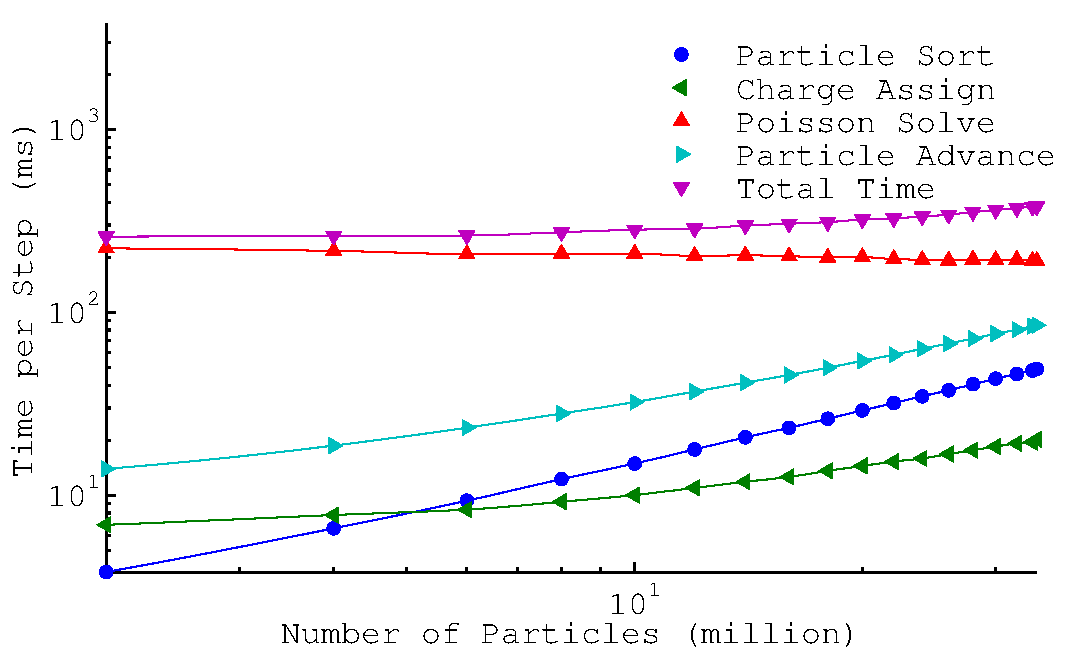
\includegraphics[width=6in]{performance/nptclsize_scan128x64x64ons8bins.pdf}
\end{center}
\caption{Number of Particles Scan on a 128x64x64 grid}
\label{fig:nptclsize_scan128x64x64}
\end{figure}

\begin{figure}[h]
\begin{center}
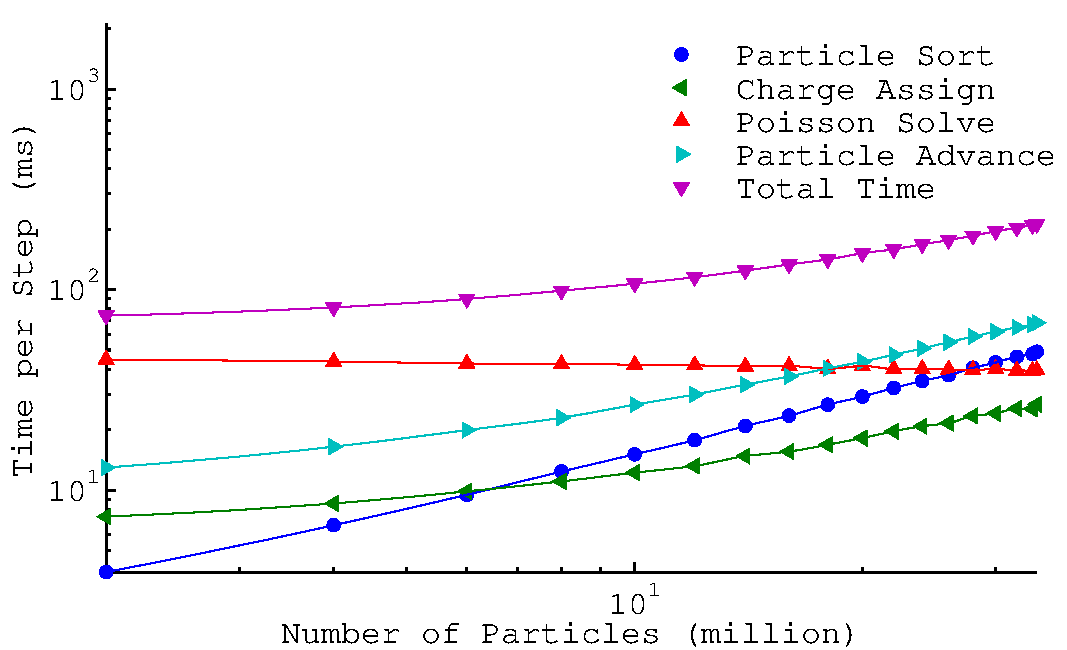
\includegraphics[width=6in]{performance/nptclsize_scan64x32x32ons8bins.pdf}
\end{center}
\caption{Number of Particles Scan on a 64x32x32 grid}
\label{fig:nptclsize_scan64x32x32}
\end{figure}

\begin{figure}[h]
\begin{center}
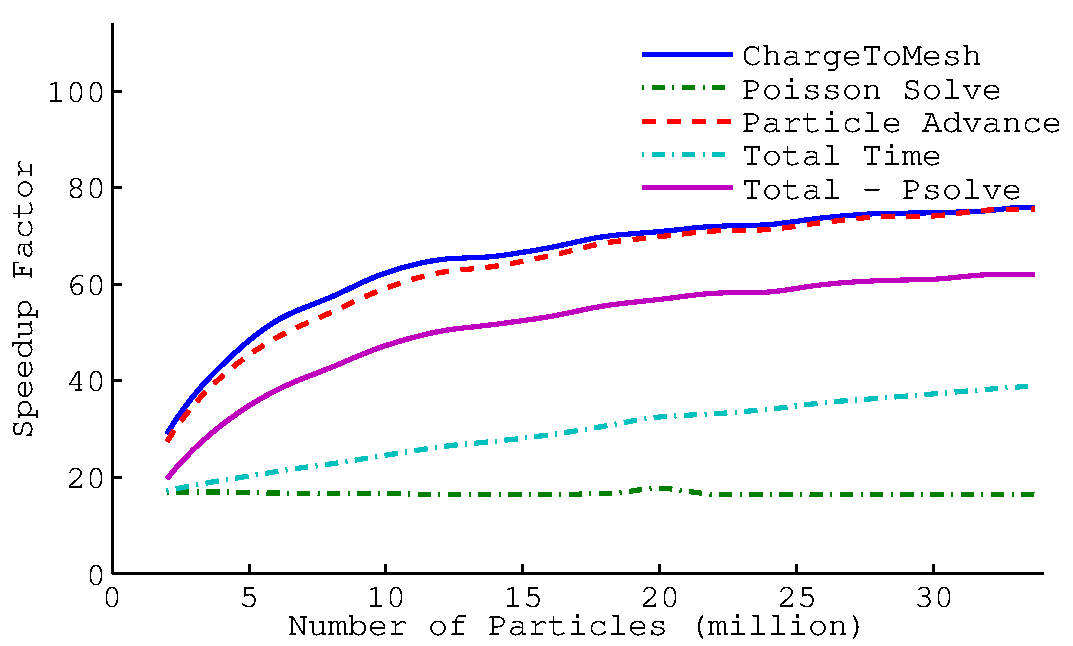
\includegraphics[width=6in]{performance/nptclspeedup_scan128x64x64ons8bins.pdf}
\end{center}
\caption{Speedup factor Number of Particles Scan on a 128x64x64 grid}
\label{fig:nptclsize_scan_speedup}
\end{figure}


	
	\section{Grid Size scan}
		\subsection{Absolue Size}
\begin{figure}[h]
\begin{center}
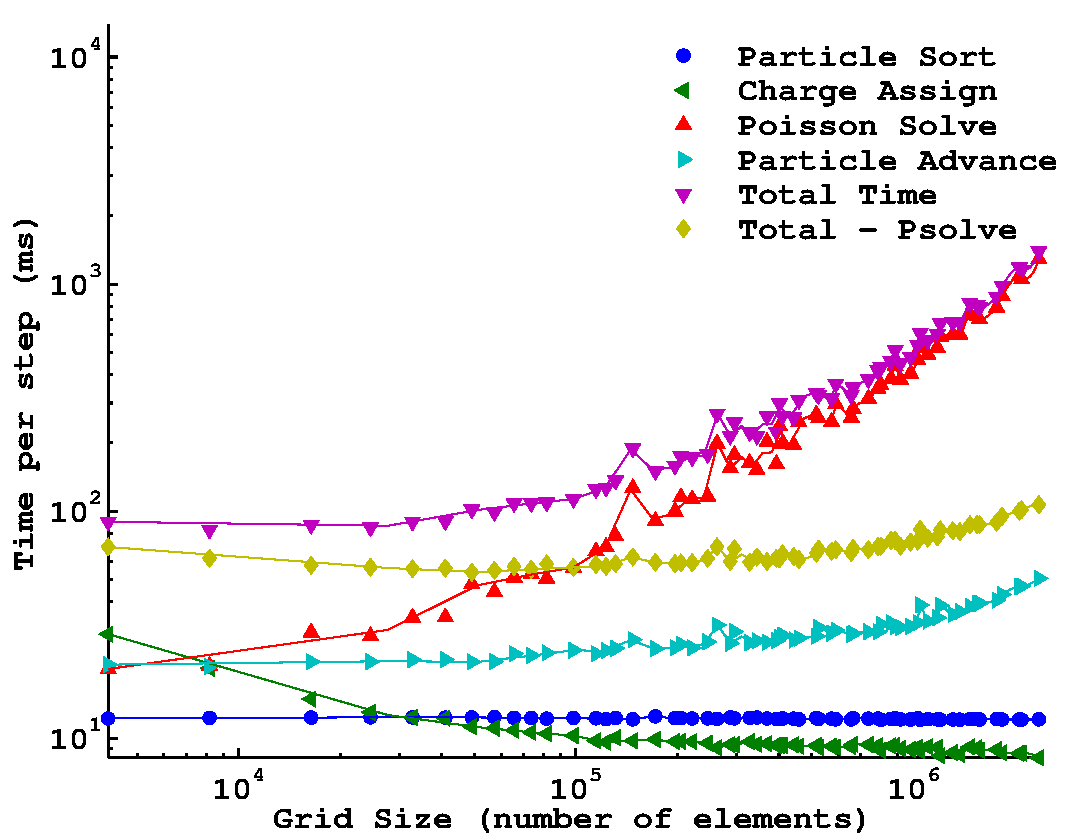
\includegraphics[width=6in]{performance/gridsize_scan8ptcls8bins.pdf}
\end{center}
\caption{Gridsize Scan with 8 million ptcls, and $8^3$ bins}
\label{fig:nptclsize_scan128x64x64}
\end{figure}


\begin{figure}[h]
\begin{center}

\includegraphics[width=6in]{performance/gridsize_scan8ptcls16bins.pdf}
\end{center}
\caption{Gridsize Scan with 8 million ptcls, and $16^3$ bins}
\label{fig:nptclsize_scan128x64x64}
\end{figure}


\begin{figure}[h]
\begin{center}
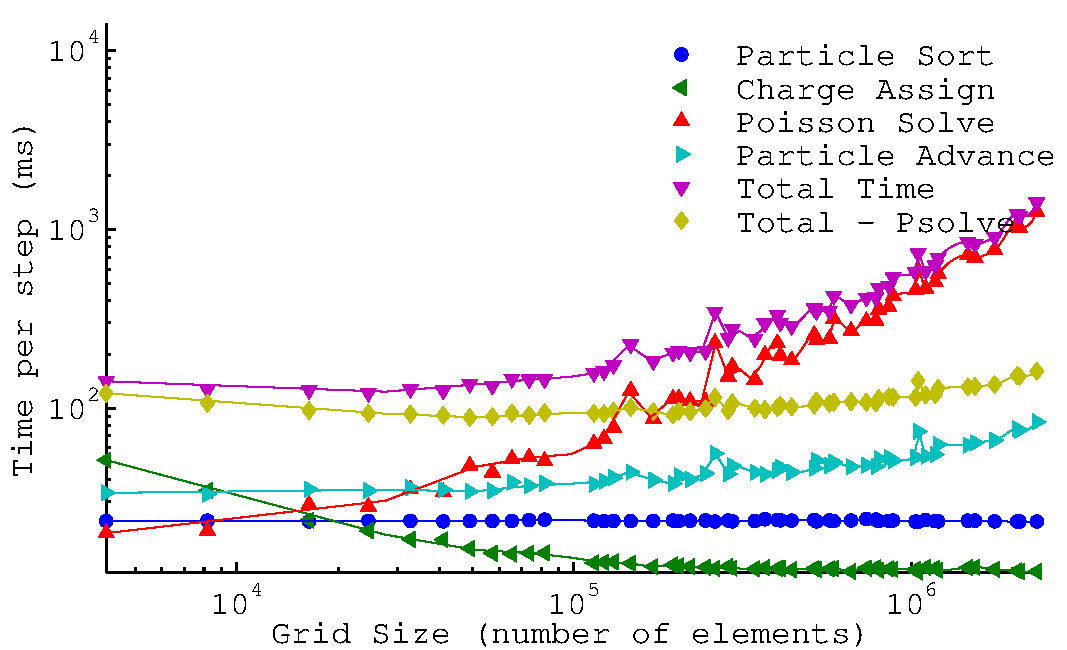
\includegraphics[width=6in]{performance/gridsize_scan16ptcls8bins.pdf}
\end{center}
\caption{Gridsize Scan with 16 million ptcls, and $8^3$ bins}
\label{fig:nptclsize_scan128x64x64}
\end{figure}

\begin{figure}[h]
\begin{center}
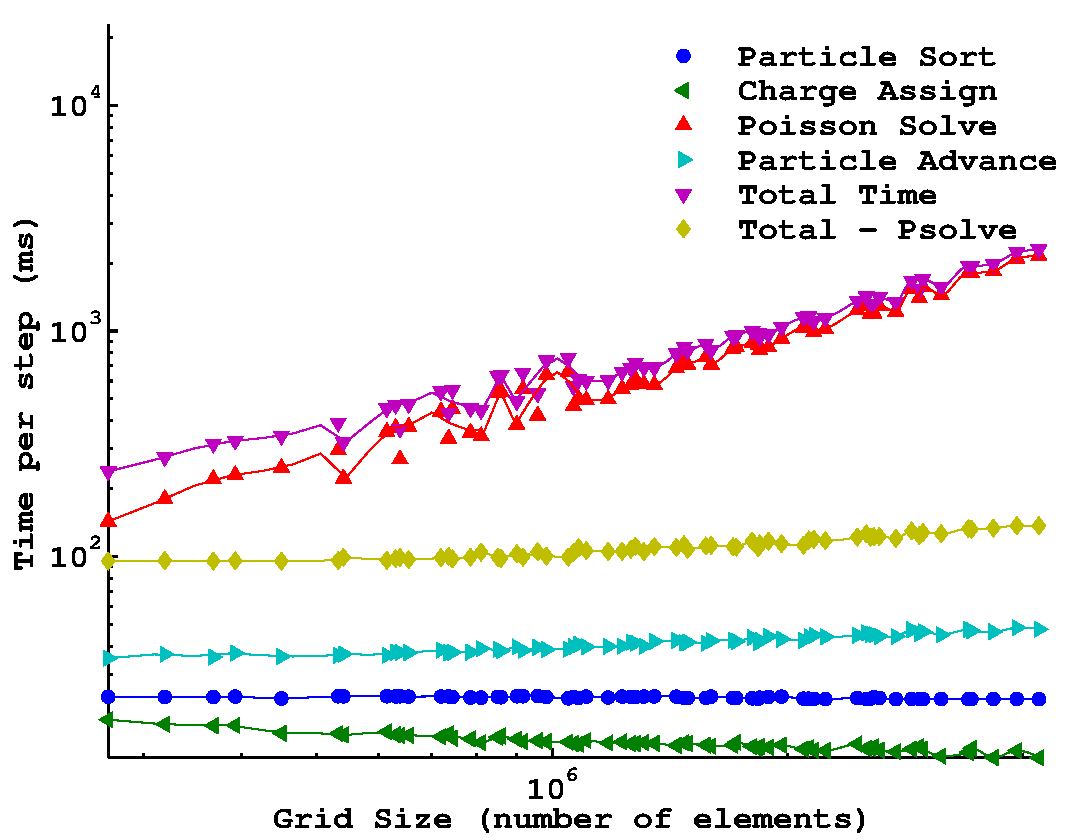
\includegraphics[width=6in]{performance/gridsize_scan16ptcls16bins.pdf}
\end{center}
\caption{Gridsize Scan with 16 million ptcls, and $16^3$ bins}
\label{fig:nptclsize_scan128x64x64}
\end{figure}

\begin{figure}[h]
\begin{center}
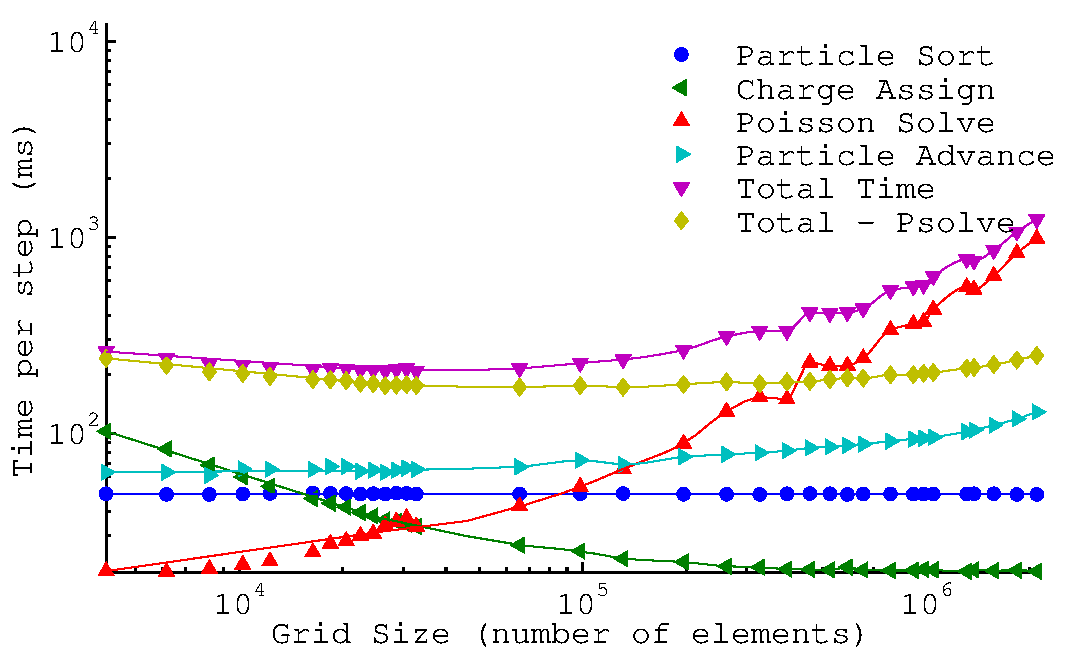
\includegraphics[width=6in]{performance/gridsize_scan34ptcls8bins.pdf}
\end{center}
\caption{Gridsize Scan with 34 million ptcls, and $8^3$ bins. Note how when the contribution from the poisson solve is removed there is a clear minimum at about $10^5$ elements. }
\label{fig:nptclsize_scan128x64x64}
\end{figure}

\begin{figure}[h]
\begin{center}
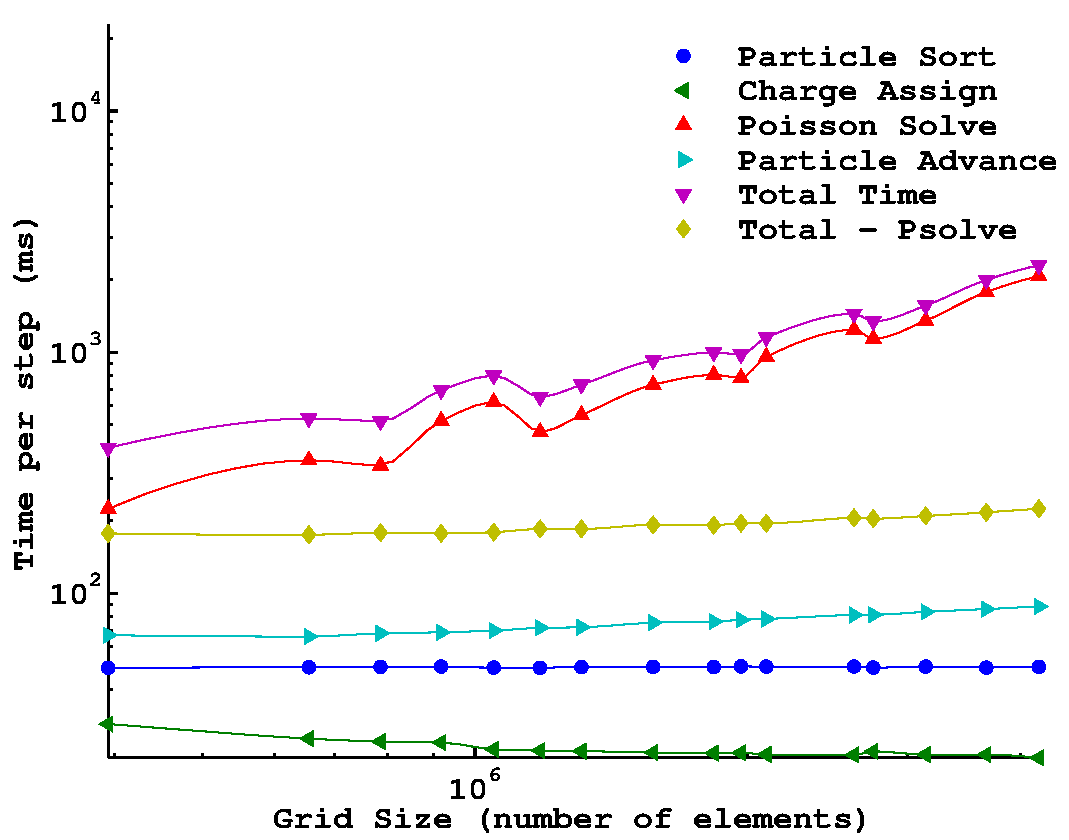
\includegraphics[width=6in]{performance/gridsize_scan34ptcls16bins.pdf}
\end{center}
\caption{Gridsize Scan with 34 million ptcls, and $16^3$ bins}
\label{fig:nptclsize_scan128x64x64}
\end{figure}


		\subsection{Ratio of Surface Area to Volume}
\begin{figure}[h]
\begin{center}
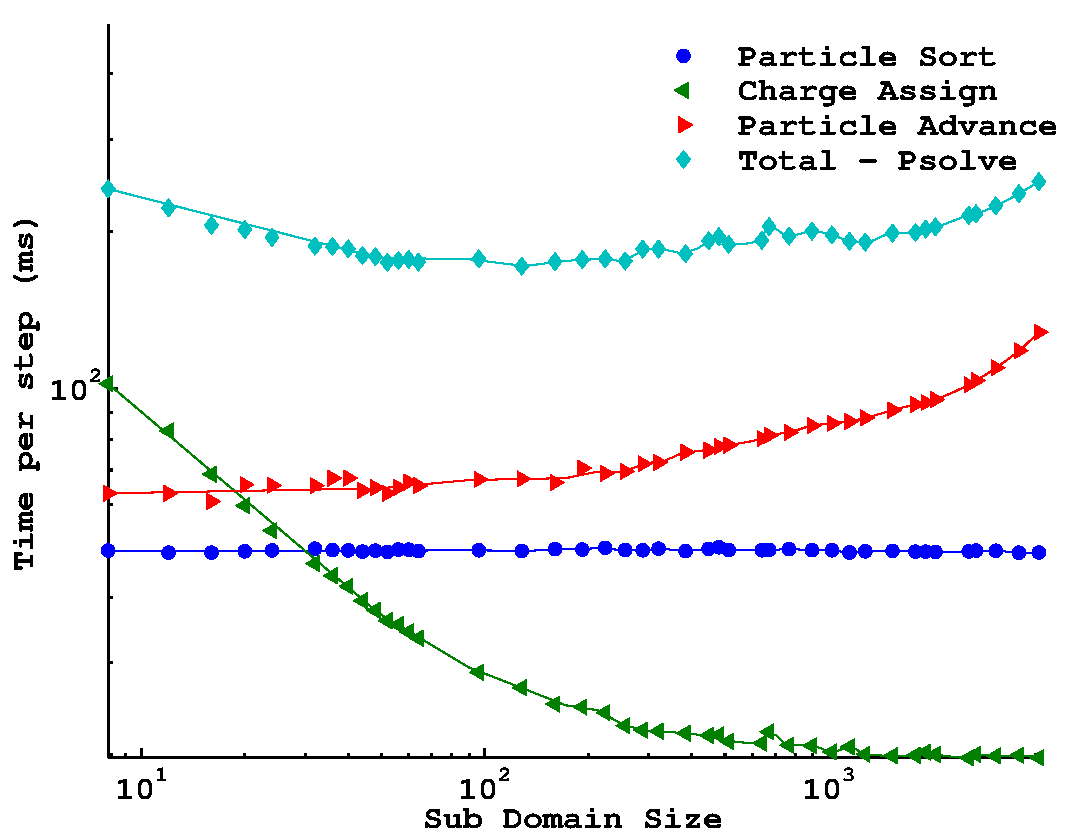
\includegraphics[width=6in]{performance/gridshape_scan.pdf}
\end{center}
\caption{Sub Domain Size scan, also known as bin size, note the minimum in the total - psolve run time.}
\label{fig:subdomain_size_scan}
\end{figure}

			\subsubsection{Global Domain Ratio}
			\subsubsection{Threadblock Sub-Domain Ratio}

	\section{Kernel Parameters Scan}

	\section{Discussion}
